\chapter{Conductors and Superconductors}\label{ch:MaterialScience}

This chapter starts by considering how normal conductors and superconductors respond to AC and DC fields. Surface resistance is defined for conductors and superconductors under the operating conditions of axion detectors. With a fundamental understanding of superconductors, thin films of superconducting materials can be coated on the inner surfaces of cavities to achieve high-$Q$ at high fields. 

\section{Normal Conductors}
    
    \subsection{Static Field}
    
    This discussion of conductors follows from Ashcroft and Mermin~\cite{ashcroftSolidStatePhysics1976}. The behavior of metals can be predicted and described using the free electron model. This simple model assumes that an atom's outer electrons are free to wander in the metal ion lattice. When these electrons sense an electric field, they move due to the force $\mathbf{F}=e\mathbf{E}$. The electrons may scatter off impurities, phonons (lattice vibrations), or other electrons, leading to an average time between collisions $\tau$. The mean free path $\ell = v_F\tau$ (where $v_F$ is the Fermi velocity) characterizes the average distance an electron travels between collisions. The equation of motion for the electron is
    
    \begin{align}
        m\frac{dv_d}{dt} = -e\mathbf{E}(t) - \frac{m}{\tau}v_d\label{eq:EOMcondcutor}
    \end{align}   

    \noindent where $m$ is the electron mass, $e$ is the electron charge, and $v_d$ is the drift velocity. The first term $-e\mathbf{E}(t)$ represents the driving force, while the second term $- \frac{m}{\tau}v_d$ represents dissipation from scattering. With the constant DC electric field, the steady-state drift velocity is
    
    \begin{align}
        v_d = \frac{eE\tau}{m}\,. \label{eq:driftvelocity}
    \end{align}
    
    \noindent These electrons are charged particles, so moving through the material creates a measurable current in the material:
    
    \begin{align}
        \mathbf{j} = -ne\mathbf{v}_d\,, \label{eq:normalcurrent}
    \end{align}
    
    \noindent where $n$ is the number density of conduction electrons. Combining equations~\ref{eq:driftvelocity},~\ref{eq:normalcurrent}, and $J=\sigma \textbf{E}$ yields the DC electrical conductivity $\sigma$ or resistivity $\rho$: 
    
    \begin{align}
        \sigma = \frac{1}{\rho} = \frac{ne^2\tau}{m} \,. \label{eq:normalconductivity}
    \end{align}

    As the material temperature decreases, thermal oscillations (phonons) decrease, leading to reduced electron scattering and lower resistivity. At low temperature $T < 20$~K, phonons freeze out, and $\rho$ saturates to a residual resistance related to the purity of the material (Fig.~\ref{fig:RRRResistivity}). The purity is quantified with the residual resistivity ratio (RRR), defined as the ratio between room temperature and residual resistivity (resistivity value saturating at $T = 0$~K):
    
    \begin{align}
        RRR = \frac{\rho(300~\text{K})}{\rho_0}. \label{eq:RRR}
    \end{align}

    \noindent The electrical conductivity of high purity Cu (RRR = 300) is $\sigma \approx 2 \times10^{10}$ S/m.
    
    \begin{figure}
        \centering
        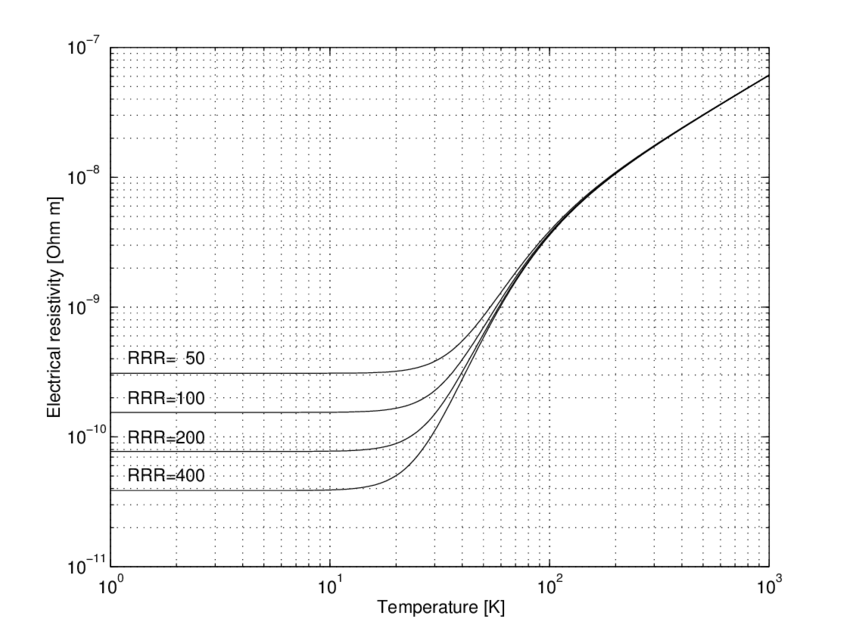
\includegraphics[width=.75\textwidth]{images/intro/RRRResistivity.png}
        \caption{Resistivity of Cu with varying levels of purity (Residual resistivity ratio - RRR) as a function of temperature~\cite{krainzQuenchProtectionPowering1997}.}
        \label{fig:RRRResistivity}
    \end{figure}
    
    \FloatBarrier
    
    \subsection{Classical Skin Effect in AC field}

    Conductors resist the penetration of time-varying magnetic fields (AC-currents) by inducing eddy currents in the conductor. These currents concentrate near the surface over a characteristic depth called the skin depth~\cite{johndavidjacksonClassicalElectrodynamicsThird1999}:

    \begin{align}
        \delta = \frac{1}{\sqrt{\pi f \mu_0 \sigma}} \label{eq:skindepth}
    \end{align}
    
    \noindent where $f$ is the AC frequency and $\mu_0=4 \pi\times10^{-7}$~H/m is the permeability of free space. For copper, the skin depth at 300~K and 10~GHz is $\approx 0.6$~\unit{\um}. With these currents restricted to the conductor surface, the usable cross-sectional area of the conductor is reduced, leading to higher resistance. This is modeled as a current flowing through a thin resistive square sheet of area $L\times L$ and thickness $\delta$. The surface resistance is

    

    \begin{align}
        R_s = \rho \cdot \frac{\text{length}}{\text{Cross-sectional area}} = \frac{1}{\sigma} \cdot \frac{L}{L \cdot \delta}\,,
       \label{eq:SurfaceResistance1}
    \end{align}

    \noindent which, substituting Eq.~\ref{eq:skindepth}, simplifies to:

    \begin{align}
        R_s = \sqrt{\frac{\pi f \mu_0}{\sigma}} \,.
       \label{eq:SurfaceResistance2}
    \end{align}

    \begin{comment}
 
    \subsection{Surface Impedance: Dissipation and Inertia}
    
    The complete AC response of a conductor includes both resistive and reactive components. Solving Eq.~\ref{eq:EOMcondcutor} for an AC field $\mathbf{E}(t) = \mathbf{E}_0 e^{i\omega t}$ in the typical microwave regime where $\omega\tau \ll 1$ gives real and imaginary components to the surface impedance, which is the sum of both resistive and reactive components
    
    \begin{align}
    Z_s = R_s + iX_s .\label{eq:normalsurfaceimpedance}
    \end{align}
    
    \noindent $R_s$ represents energy dissipation from electron collisions (resistance) and $X_s$ represents the inductive response from electron inertia (reactance). For normal metals at microwave frequencies, the resistive and reactive contributions are equal:
    
    \begin{align}
        R_s = X_s = \sqrt{\frac{\pi f \mu_0}{\sigma}} .\label{eq:RsXsequal}
    \end{align}
    
    \noindent The resistive component is dominated by electrons scattering in the skin depth of the material, and is therefore dependent on conductivity.
       
    \end{comment}


    \subsection{Anomalous Skin Depth}

    At low-temperature $T<20$~K and high-frequency $f>100$~MHz, the classical skin depth equation~\ref{eq:SurfaceResistance2} doesn't hold, and the surface resistance no longer depends on conductivity~\cite{pippardf.r.s.SurfaceImpedanceSuperconductors1947}. This anomalous skin-depth regime can be attributed to the skin depth becoming smaller than the scattering length, i.e., $\ell > \delta$. As the electrons travel through the skin depth, they no longer scatter at the same rate. This reduces the conductor's effectiveness at AC-field screening, leading to increased surface resistance. The effective anomalous skin depth is defined as~\cite{Braine:2024nzi}:

    \begin{align}
        \delta_{\text{anom}} = \left(\frac{\sqrt3c^2 m v_F}{8\pi^2 \omega_0 n e^2}\right)^{1/3} , \label{eq:anomalousskin}
    \end{align}

    \noindent For Cu, $v_F = 1.57 \times 10^8$ cm/s and $n = 8.50 \times 10^{22}$ cm$^{-3}$, which simplifies the above equation to:
    
    \begin{align}
        \delta_{\text{anom,Cu}} = 2.84 \times 10^{-4} \text{ m} \left(\frac{1}{f}\right)^{1/3} \, \label{eq:anomalouscopperskin}
    \end{align}

    \noindent with frequency in Hz. For copper at 10~GHz and 20~K, the effective skin depth is $\approx0.2$~\unit{\um}.

    Most electromagnetic simulation software (COMSOL, ANSYS) assumes the classical skin effect. To use these modeling tools in the anomalous regime, an effective conductivity $\sigma_{\text{eff}}$ can be defined that reproduces the correct surface resistance when inserted into the classical formula $R_s = \sqrt{\pi f \mu_0 / \sigma_{\text{eff}}}$.

    Starting from the requirement that $R_s = 1/(\sigma_{\text{eff}} \,\delta_{\text{anom}})$ must equal the classical form Eq.~\ref{eq:SurfaceResistance2}, the effective conductivity for Cu at cryogenic temperatures becomes 
    
    \begin{align}
        \sigma_{\text{eff,anom,Cu}} = \frac{1}{2\mu_0 c \pi f \delta_{\text{anom}}^2} = 3.14 \times 10^{12} \text{ S/m} \cdot f^{-1/3} \,.\label{eq:effectiveconductivity}
    \end{align}

    \noindent While DC conductivity improves 340$\times$ from room temperature to  4~K, the anomalous skin effect reduces this benefit to $5-20\times$ improvement (Table~\ref{tab:sigma_eff_anomalous}). This frequency-dependent degradation becomes more severe at higher frequencies~\cite{padamseeRFSuperconductivity2009}.

    


    %When copper cavities are cooled from room temperature to 100 mK, the DC resistivity decreases by a factor of 100, but the surface resistance only decreases by a factor of 6~\cite{padamseeRFSuperconductivity2009}.

    The anomalous skin effect leads to a stronger frequency dependence on surface resistance, where $R_s \propto f^{2/3}$, compared to the classical $R_s \propto f^{1/2}$ scaling. Calculating surface resistance and quality factor in this anomalous regime with equations~\ref{eq:SurfaceResistance2} and~\ref{eq:effectiveconductivity}, we find that $Q$ drops by $\sim 75\%$ from 1-10 GHz (seen in table~\ref{tab:Rs_Q_anomalous}). The strong degradation in $Q$ with frequency becomes problematic as axion searches push beyond $10$~GHz ($m_a \sim 10^{-5}$~eV). Conductors have remained the material of choice for high-field RF applications due to their surface resistance degrading very weakly in large magnetic fields. 


    \begin{table}[ht]
        \centering
        \caption{Conductivity of Cu (high-purity, RRR=300) at 4~K showing degradation from anomalous skin effect}
        \label{tab:sigma_eff_anomalous}
        \begin{tabular}{ccc}
        \toprule
        \textbf{Frequency (GHz)} & \textbf{$\bm{\sigma}$ or $\bm{\sigma_{\text{eff}}}$ (S/m)} & \textbf{Improvement from 300~K} \\
        \midrule
        DC & $2.0 \times 10^{10}$ & 340$\times$ \\
        \midrule
        1  & $3.14 \times 10^9$ & 54$\times$ \\
        5  & $1.84 \times 10^9$ & 32$\times$ \\
        10 & $1.46 \times 10^9$ & 25$\times$ \\
        20 & $1.16 \times 10^9$ & 20$\times$ \\
        \bottomrule
        \end{tabular}
    \end{table}


  \begin{table}[ht]
        \centering
        \caption{Theoretical best surface resistance and quality factor for Cu (high-purity, RRR=300) at 4~K in the anomalous regime ($G = 350~\Omega$)}
        \label{tab:Rs_Q_anomalous}
        \begin{tabular}{ccc}
        \toprule
        \textbf{Frequency (GHz)} & \textbf{$\bm{R_s}$ (m$\bm{\Omega}$)} & \textbf{$\bm{Q}$} \\
        \midrule
        1  & 1 & 300{,}000 \\
        5  & 3 & 100{,}000 \\
        10 & 5 & 70{,}000 \\
        20 & 8 & 40{,}000 \\
        \bottomrule
    \end{tabular}
    \end{table}

\input{Chapters/3_2Superconductors}
